\documentclass[aspectratio=169,11pt]{beamer}

% ── Theme ────────────────────────────────────────────────────────
\usetheme{Madrid}
\usecolortheme{default}
\definecolor{MSTANgreen}{RGB}{16,185,129}
\definecolor{DarkBg}{RGB}{30,41,59}
\setbeamercolor{structure}{fg=MSTANgreen}
\setbeamercolor{palette primary}{bg=DarkBg,fg=white}
\setbeamercolor{palette secondary}{bg=DarkBg!90,fg=white}
\setbeamercolor{palette tertiary}{bg=MSTANgreen,fg=white}
\setbeamercolor{title}{fg=white,bg=DarkBg}
\setbeamercolor{frametitle}{fg=white,bg=DarkBg}
\setbeamercolor{block title}{bg=MSTANgreen!90,fg=white}
\setbeamercolor{block body}{bg=MSTANgreen!8}
\setbeamercolor{block title alerted}{bg=red!70!black,fg=white}
\setbeamercolor{block body alerted}{bg=red!5}
\setbeamercolor{block title example}{bg=DarkBg!80,fg=white}
\setbeamercolor{block body example}{bg=DarkBg!5}
\setbeamertemplate{navigation symbols}{}
\setbeamertemplate{footline}{
  \leavevmode\hbox{%
    \begin{beamercolorbox}[wd=.33\paperwidth,ht=2.5ex,dp=1ex,center]{palette primary}%
      \usebeamerfont{author in head/foot}\insertshortauthor
    \end{beamercolorbox}%
    \begin{beamercolorbox}[wd=.34\paperwidth,ht=2.5ex,dp=1ex,center]{palette secondary}%
      \usebeamerfont{title in head/foot}\insertshorttitle
    \end{beamercolorbox}%
    \begin{beamercolorbox}[wd=.33\paperwidth,ht=2.5ex,dp=1ex,right]{palette tertiary}%
      \insertframenumber{}/\inserttotalframenumber\hspace*{2ex}
    \end{beamercolorbox}}%
}

% ── Packages ─────────────────────────────────────────────────────
\usepackage[utf8]{inputenc}
\usepackage[T1]{fontenc}
\usepackage{amsmath,amssymb}
\usepackage{booktabs}
\usepackage{graphicx}
\usepackage{tikz}
\usetikzlibrary{arrows.meta,positioning,shapes.geometric,calc,fit}
\usepackage{xcolor}
\usepackage{hyperref}
\usepackage{multicol}
\usepackage{caption}
\captionsetup[figure]{font=scriptsize,labelfont=scriptsize}

% ── Meta ─────────────────────────────────────────────────────────
\title[Churn AI — MSTAN]{Deep Learning--Driven Customer Churn Forecasting\\[4pt]
\small A Multi-Scale Temporal Attention Network Approach}
\author[Your Name]{Your Name\\[2pt]
{\scriptsize Supervisor: Prof.\ Supervisor Name}}
\institute[Dept]{Department of Computer Science \& Engineering\\Your University}
\date{Final Year Project Presentation \\ March 2026}

% ══════════════════════════════════════════════════════════════════
\begin{document}

% ── Title ────────────────────────────────────────────────────────
\begin{frame}[plain]
\titlepage
\end{frame}

% ── Outline ──────────────────────────────────────────────────────
\begin{frame}{Outline}
\tableofcontents
\end{frame}

% ══════════════════════════════════════════════════════════════════
\section{Introduction \& Motivation}
% ══════════════════════════════════════════════════════════════════

\begin{frame}{The Business Problem}
\begin{columns}[T]
\begin{column}{0.55\textwidth}
\begin{itemize}
    \item \textbf{Customer churn} — when a subscriber stops using a service — costs telecom companies \textbf{billions annually}.
    \item Acquiring a new customer costs \textbf{5--25$\times$} more than retaining an existing one \cite{reichheld1996}.
    \item Early identification of at-risk customers enables \textbf{proactive retention} interventions.
\end{itemize}
\vspace{6pt}
\begin{alertblock}{Key Challenge}
Traditional ML approaches treat customer records as \textbf{static snapshots}, ignoring the \emph{temporal evolution} of customer behaviour.
\end{alertblock}
\end{column}
\begin{column}{0.42\textwidth}
\centering
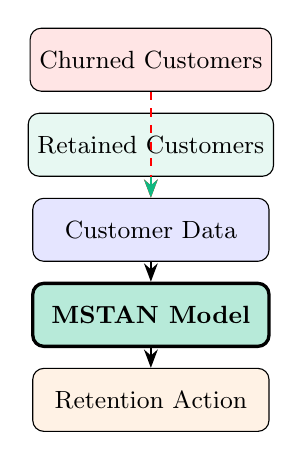
\begin{tikzpicture}[scale=0.72, every node/.style={font=\small}]
    \node[draw, rounded corners, fill=red!10, minimum width=3cm, minimum height=0.8cm] (churn) at (0,3) {Churned Customers};
    \node[draw, rounded corners, fill=MSTANgreen!10, minimum width=3cm, minimum height=0.8cm] (retain) at (0,1.5) {Retained Customers};
    \node[draw, rounded corners, fill=blue!10, minimum width=3cm, minimum height=0.8cm] (data) at (0,0) {Customer Data};
    \node[draw, rounded corners, fill=MSTANgreen!30, minimum width=3cm, minimum height=0.8cm, line width=1.2pt] (model) at (0,-1.5) {\textbf{MSTAN Model}};
    \node[draw, rounded corners, fill=orange!10, minimum width=3cm, minimum height=0.8cm] (action) at (0,-3) {Retention Action};
    \draw[-{Stealth}, thick] (data) -- (model);
    \draw[-{Stealth}, thick] (model) -- (action);
    \draw[-{Stealth}, thick, dashed, red] (churn) -- (data);
    \draw[-{Stealth}, thick, dashed, MSTANgreen] (retain) -- (data);
\end{tikzpicture}
\end{column}
\end{columns}
\end{frame}

% ──────────────────────────────────────────────────────────────────
\begin{frame}{Why Temporal Modelling?}
\begin{columns}[T]
\begin{column}{0.55\textwidth}
Customer churn is a \textbf{process, not an event}:
\begin{enumerate}
    \item Monthly charges \textbf{gradually increase}
    \item Support service usage \textbf{declines}
    \item Contract changes from long-term to \textbf{month-to-month}
    \item Customer eventually \textbf{churns}
\end{enumerate}
\vspace{6pt}
\begin{exampleblock}{Our Insight}
Modelling \emph{how} customer features change over time — not just their current values — can reveal churn \textbf{before} it happens.
\end{exampleblock}
\end{column}
\begin{column}{0.42\textwidth}
\centering
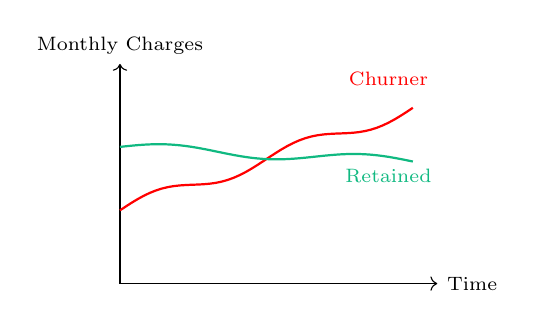
\begin{tikzpicture}[scale=0.62]
    % Churner trajectory
    \draw[->] (0,0) -- (6.5,0) node[right, font=\scriptsize] {Time};
    \draw[->] (0,0) -- (0,4.5) node[above, font=\scriptsize] {Monthly Charges};
    \draw[thick, red, domain=0:6, samples=50] plot (\x, {1.5 + 0.35*\x + 0.15*sin(120*\x)});
    \draw[thick, MSTANgreen, domain=0:6, samples=50] plot (\x, {2.8 - 0.05*\x + 0.1*sin(90*\x)});
    \node[font=\scriptsize, red] at (5.5, 4.2) {Churner};
    \node[font=\scriptsize, MSTANgreen] at (5.5, 2.2) {Retained};
\end{tikzpicture}
\end{column}
\end{columns}
\end{frame}

% ──────────────────────────────────────────────────────────────────
\begin{frame}{Objectives}
\begin{enumerate}
    \item Design a \textbf{novel deep learning architecture} (MSTAN) that captures multi-scale temporal patterns in customer behaviour.
    \item Handle \textbf{class imbalance} (26.5\% churn rate) using Focal Loss.
    \item Perform a \textbf{rigorous comparative study} against 4 baseline models under controlled experimental conditions.
    \item Build an \textbf{interactive deployment dashboard} for real-time churn prediction.
\end{enumerate}
\end{frame}

% ══════════════════════════════════════════════════════════════════
\section{Literature Review}
% ══════════════════════════════════════════════════════════════════

\begin{frame}{Literature Review — Traditional Approaches}
\begin{table}[h]
\centering
\small
\begin{tabular}{p{3.2cm} p{4.5cm} p{4.5cm}}
\toprule
\textbf{Reference} & \textbf{Method} & \textbf{Limitation} \\
\midrule
Amin et al.\ (2019) \cite{amin2019} & Logistic Regression, SVM with data certainty & Static features only; no temporal dynamics \\[4pt]
De Caigny et al.\ (2018) \cite{decaigny2018} & Hybrid logistic regression + decision trees & Limited to linear feature interactions \\[4pt]
Lalwani et al.\ (2022) \cite{lalwani2022} & Random Forest, XGBoost ensemble & No sequential modelling; ignores feature evolution \\
\bottomrule
\end{tabular}
\end{table}
\vspace{4pt}
\begin{alertblock}{Gap}
All treat each customer as a \textbf{single static vector} — temporal behaviour is discarded.
\end{alertblock}
\end{frame}

% ──────────────────────────────────────────────────────────────────
\begin{frame}{Literature Review — Deep Learning Approaches}
\begin{table}[h]
\centering
\small
\begin{tabular}{p{3.2cm} p{4.5cm} p{4.5cm}}
\toprule
\textbf{Reference} & \textbf{Method} & \textbf{Limitation} \\
\midrule
Fujo et al.\ (2022) \cite{fujo2022} & LSTM/GRU for sequential churn & Single temporal scale; no multi-resolution \\[4pt]
Wen et al.\ (2023) \cite{wen2023} & Transformers in time series (survey) & Standard attention treats all timesteps equally \\[4pt]
Lim et al.\ (2021) \cite{lim2021} & Temporal Fusion Transformer & Designed for multi-horizon forecasting, not classification \\
\bottomrule
\end{tabular}
\end{table}
\vspace{4pt}
\begin{alertblock}{Gap}
No existing work combines \textbf{multi-scale temporal convolutions} with \textbf{recency-biased attention} for churn prediction.
\end{alertblock}
\end{frame}

% ──────────────────────────────────────────────────────────────────
\begin{frame}{Literature Review — Key Architectural Foundations}
\begin{table}[h]
\centering
\small
\begin{tabular}{p{3.2cm} p{4.5cm} p{4cm}}
\toprule
\textbf{Reference} & \textbf{Contribution} & \textbf{Our Use} \\
\midrule
Bai et al.\ (2018) \cite{bai2018} & Temporal Convolutional Networks (TCN) & Dilated causal convolutions \\[4pt]
Press et al.\ (2022) \cite{press2022} & ALiBi — linear attention bias & Inspires temporal decay bias \\[4pt]
Lin et al.\ (2017) \cite{lin2017} & Focal Loss & Class imbalance handling \\[4pt]
Fawaz et al.\ (2020) \cite{fawaz2020} & InceptionTime — multi-scale convolutions & Multi-resolution feature extraction \\
\bottomrule
\end{tabular}
\end{table}
\end{frame}

% ──────────────────────────────────────────────────────────────────
\begin{frame}{Research Gap \& Our Contribution}
\begin{block}{Research Gap}
Existing churn prediction methods either (1) use static features ignoring temporal dynamics, (2) apply single-scale sequential models (LSTM/GRU), or (3) use standard Transformers that treat all timesteps equally. \textbf{No prior work} combines multi-scale temporal feature extraction with decay-biased attention for churn.
\end{block}
\vspace{8pt}
\textbf{Our Contributions:}
\begin{enumerate}
    \item \textbf{MSTAN} — a novel architecture combining multi-scale temporal convolutions with gated fusion and \emph{learnable} temporal decay attention bias.
    \item \textbf{Churn-correlated temporal sequence synthesis} — transforming static records into label-aware behavioural trajectories.
    \item \textbf{Comprehensive comparative framework} — 5 models, Focal Loss, F1-optimal thresholds, and an interactive deployment dashboard.
\end{enumerate}
\end{frame}

% ══════════════════════════════════════════════════════════════════
\section{Dataset \& Preprocessing}
% ══════════════════════════════════════════════════════════════════

\begin{frame}{Dataset — IBM Telco Customer Churn}
\begin{columns}[T]
\begin{column}{0.50\textwidth}
\begin{itemize}
    \item \textbf{Source:} IBM Sample Datasets (Kaggle)
    \item \textbf{Records:} 7,043 customers
    \item \textbf{Features:} 19 (16 categorical + 3 numerical)
    \item \textbf{Target:} Binary — Churn (Yes/No)
    \item \textbf{Class distribution:} 73.5\% No / \textcolor{red}{26.5\% Yes}
\end{itemize}
\vspace{4pt}
\begin{exampleblock}{Key Features}
\texttt{tenure}, \texttt{MonthlyCharges}, \texttt{TotalCharges}, \texttt{Contract}, \texttt{InternetService}, \texttt{PaymentMethod}, ...
\end{exampleblock}
\end{column}
\begin{column}{0.47\textwidth}
\centering
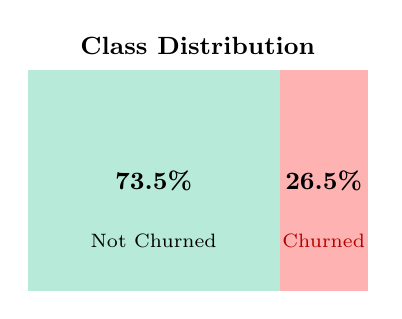
\begin{tikzpicture}[scale=0.8]
    \fill[MSTANgreen!30] (0,0) rectangle (4, 3.5);
    \fill[red!30] (4,0) rectangle (5.4, 3.5);
    \node[font=\small\bfseries] at (2, 1.75) {73.5\%};
    \node[font=\small\bfseries] at (4.7, 1.75) {26.5\%};
    \node[font=\scriptsize] at (2, 0.8) {Not Churned};
    \node[font=\scriptsize, red!70!black] at (4.7, 0.8) {Churned};
    \node[font=\small\bfseries, above] at (2.7, 3.6) {Class Distribution};
\end{tikzpicture}
\\[10pt]
\small \textbf{Imbalance ratio:} $\approx$ 2.8 : 1
\end{column}
\end{columns}
\end{frame}

% ──────────────────────────────────────────────────────────────────
\begin{frame}{Preprocessing Pipeline}
\begin{center}
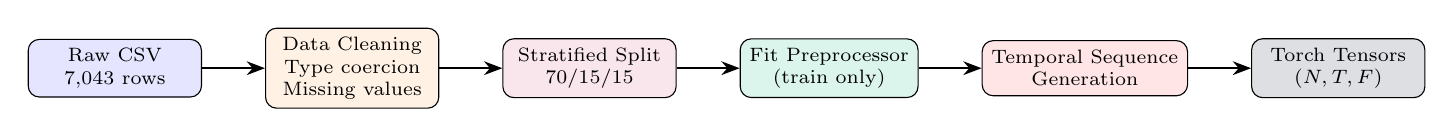
\begin{tikzpicture}[
    node distance=0.6cm and 0.8cm,
    box/.style={draw, rounded corners, minimum width=2.2cm, minimum height=0.7cm, font=\scriptsize, align=center},
    arrow/.style={-{Stealth}, thick}
]
    \node[box, fill=blue!10] (raw) {Raw CSV\\7,043 rows};
    \node[box, fill=orange!10, right=of raw] (clean) {Data Cleaning\\Type coercion\\Missing values};
    \node[box, fill=purple!10, right=of clean] (split) {Stratified Split\\70/15/15};
    \node[box, fill=MSTANgreen!15, right=of split] (encode) {Fit Preprocessor\\(train only)};
    \node[box, fill=red!10, right=of encode] (seq) {Temporal Sequence\\Generation};
    \node[box, fill=DarkBg!15, right=of seq] (tensor) {Torch Tensors\\$(N, T, F)$};
    
    \draw[arrow] (raw) -- (clean);
    \draw[arrow] (clean) -- (split);
    \draw[arrow] (split) -- (encode);
    \draw[arrow] (encode) -- (seq);
    \draw[arrow] (seq) -- (tensor);
\end{tikzpicture}
\end{center}
\vspace{6pt}
\begin{columns}[T]
\begin{column}{0.48\textwidth}
\textbf{Encoding:}
\begin{itemize}
    \item Categorical $\rightarrow$ One-Hot Encoding
    \item Numerical $\rightarrow$ Standard Scaling ($\mu{=}0, \sigma{=}1$)
    \item Fitted on \textbf{training set only} (no data leakage)
\end{itemize}
\end{column}
\begin{column}{0.48\textwidth}
\textbf{Final Dimensions:}
\begin{itemize}
    \item Feature dimension: $F = 46$
    \item Sequence length: $T = 12$ timesteps
    \item Train: 4,930 / Val: 1,056 / Test: 1,057
\end{itemize}
\end{column}
\end{columns}
\end{frame}

% ──────────────────────────────────────────────────────────────────
\begin{frame}{Churn-Correlated Temporal Sequence Generation}
\begin{block}{Problem}
The Telco dataset is \textbf{cross-sectional} (one row per customer). Deep temporal models require \textbf{sequential} data.
\end{block}
\vspace{4pt}
\textbf{Our Approach:} Generate label-aware temporal trajectories:
\vspace{4pt}
\begin{columns}[T]
\begin{column}{0.48\textwidth}
\textcolor{red}{\textbf{Churners:}}
\begin{itemize}
    \item Monthly charges \textbf{increasing} over time
    \item Tenure growth \textbf{stagnating}
    \item Services may \textbf{downgrade} mid-sequence
\end{itemize}
\end{column}
\begin{column}{0.48\textwidth}
\textcolor{MSTANgreen}{\textbf{Non-Churners:}}
\begin{itemize}
    \item Monthly charges \textbf{stable/decreasing}
    \item Tenure growth \textbf{healthy}
    \item Services remain \textbf{stable}
\end{itemize}
\end{column}
\end{columns}
\vspace{8pt}
\begin{exampleblock}{Key Insight}
This creates \emph{informative temporal patterns} that enable sequence models to learn behavioural dynamics rather than fitting noise.
\end{exampleblock}
\end{frame}

% ══════════════════════════════════════════════════════════════════
\section{Proposed Methodology — MSTAN}
% ══════════════════════════════════════════════════════════════════

\begin{frame}{MSTAN — Architecture Overview}
\begin{center}
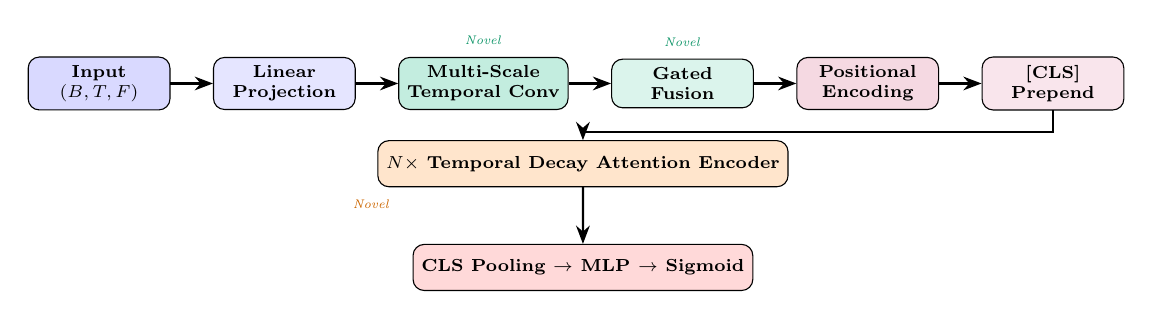
\begin{tikzpicture}[
    node distance=0.4cm and 0.5cm,
    box/.style={draw, rounded corners=4pt, minimum width=2.0cm, minimum height=0.65cm, font=\scriptsize\bfseries, align=center},
    arrow/.style={-{Stealth}, thick},
    scale=0.9, transform shape
]
    \node[box, fill=blue!15] (input) {Input\\$(B, T, F)$};
    \node[box, fill=blue!10, right=0.6cm of input] (proj) {Linear\\Projection};
    \node[box, fill=MSTANgreen!25, right=0.6cm of proj] (ms) {Multi-Scale\\Temporal Conv};
    \node[box, fill=MSTANgreen!15, right=0.6cm of ms] (gate) {Gated\\Fusion};
    \node[box, fill=purple!15, right=0.6cm of gate] (pe) {Positional\\Encoding};
    \node[box, fill=purple!10, right=0.6cm of pe] (cls) {[CLS]\\Prepend};
    
    \node[box, fill=orange!20, below=0.8cm of $(ms)!0.5!(gate)$, minimum width=5cm] (attn) {$N \times$ Temporal Decay Attention Encoder};
    \node[box, fill=red!15, below=0.8cm of attn] (pool) {CLS Pooling $\rightarrow$ MLP $\rightarrow$ Sigmoid};
    
    \draw[arrow] (input) -- (proj);
    \draw[arrow] (proj) -- (ms);
    \draw[arrow] (ms) -- (gate);
    \draw[arrow] (gate) -- (pe);
    \draw[arrow] (pe) -- (cls);
    \draw[arrow] (cls.south) -- ++(0,-0.3) -| (attn.north);
    \draw[arrow] (attn) -- (pool);
    
    % Novel labels
    \node[font=\tiny, MSTANgreen!80!black, above=0.05cm of ms] {\textit{Novel}};
    \node[font=\tiny, MSTANgreen!80!black, above=0.05cm of gate] {\textit{Novel}};
    \node[font=\tiny, orange!80!black, below left=0.05cm and -0.3cm of attn] {\textit{Novel}};
\end{tikzpicture}
\end{center}
\vspace{6pt}
\begin{columns}[T]
\begin{column}{0.32\textwidth}
\centering
\textcolor{MSTANgreen}{\textbf{Component 1}}\\
\small Multi-Scale Temporal\\Convolutions
\end{column}
\begin{column}{0.32\textwidth}
\centering
\textcolor{MSTANgreen}{\textbf{Component 2}}\\
\small Gated Feature\\Fusion
\end{column}
\begin{column}{0.32\textwidth}
\centering
\textcolor{orange!80!black}{\textbf{Component 3}}\\
\small Temporal Decay\\Attention Bias
\end{column}
\end{columns}
\end{frame}

% ──────────────────────────────────────────────────────────────────
\begin{frame}{Novel Component 1: Multi-Scale Temporal Convolutions}
\begin{columns}[T]
\begin{column}{0.52\textwidth}
\textbf{Parallel dilated causal convolutions} at scales $d \in \{1, 2, 4\}$:
\vspace{4pt}
\begin{itemize}
    \item \textbf{Scale 1:} Short-range patterns (e.g., sudden support call)
    \item \textbf{Scale 2:} Medium-range trends (e.g., service usage decline)
    \item \textbf{Scale 4:} Long-range dynamics (e.g., gradual contract downgrade)
\end{itemize}
\vspace{6pt}
Each branch: \texttt{CausalConv1d} $\rightarrow$ \texttt{GELU} $\rightarrow$ \texttt{BatchNorm}
\vspace{6pt}
\begin{exampleblock}{Why Causal?}
Left-padded convolutions ensure \textbf{no future information leakage} — predictions at time $t$ use only data from $\leq t$.
\end{exampleblock}
\end{column}
\begin{column}{0.45\textwidth}
\centering
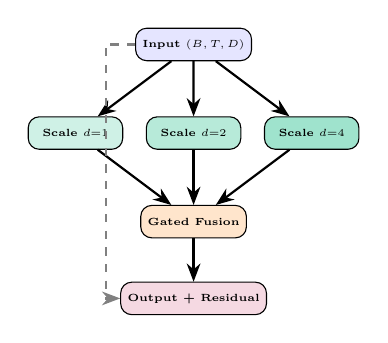
\begin{tikzpicture}[
    scale=0.75, transform shape,
    box/.style={draw, rounded corners, minimum width=1.6cm, minimum height=0.55cm, font=\tiny\bfseries, align=center},
    arrow/.style={-{Stealth}, thick}
]
    \node[box, fill=blue!10] (in) at (0,0) {Input $(B,T,D)$};
    \node[box, fill=MSTANgreen!20] (s1) at (-2, -1.5) {Scale $d{=}1$};
    \node[box, fill=MSTANgreen!30] (s2) at (0, -1.5) {Scale $d{=}2$};
    \node[box, fill=MSTANgreen!40] (s4) at (2, -1.5) {Scale $d{=}4$};
    \node[box, fill=orange!20] (gate) at (0, -3) {Gated Fusion};
    \node[box, fill=purple!15] (out) at (0, -4.3) {Output + Residual};
    
    \draw[arrow] (in) -- (s1);
    \draw[arrow] (in) -- (s2);
    \draw[arrow] (in) -- (s4);
    \draw[arrow] (s1) -- (gate);
    \draw[arrow] (s2) -- (gate);
    \draw[arrow] (s4) -- (gate);
    \draw[arrow] (gate) -- (out);
    \draw[arrow, dashed, gray] (in.west) -- ++(-0.5,0) |- (out.west);
\end{tikzpicture}
\end{column}
\end{columns}
\end{frame}

% ──────────────────────────────────────────────────────────────────
\begin{frame}{Novel Component 2: Gated Feature Fusion}
\textbf{Problem:} Different customers benefit from different temporal scales.
\vspace{6pt}

Given branch outputs $\mathbf{h}_1, \mathbf{h}_2, \mathbf{h}_4 \in \mathbb{R}^{B \times T \times D}$:
\vspace{4pt}
\begin{align}
    \mathbf{g} &= \text{softmax}\!\left(\mathbf{W}_g \cdot [\mathbf{h}_1 \| \mathbf{h}_2 \| \mathbf{h}_4]\right) \in \mathbb{R}^{B \times T \times 3} \\[4pt]
    \mathbf{h}_{\text{fused}} &= \sum_{k \in \{1,2,4\}} g_k \odot \mathbf{h}_k
\end{align}
\vspace{4pt}
\begin{itemize}
    \item The gate weights $g_k$ are \textbf{learned per-sample, per-timestep}.
    \item A customer with a \textit{slow contract downgrade} benefits from the $d{=}4$ branch.
    \item A customer with a \textit{sudden support call} benefits from the $d{=}1$ branch.
    \item The model learns to \textbf{select the optimal resolution} automatically.
\end{itemize}
\end{frame}

% ──────────────────────────────────────────────────────────────────
\begin{frame}{Novel Component 3: Temporal Decay Attention Bias}
\textbf{Intuition:} Recent customer interactions are \emph{more predictive} of churn than older ones.
\vspace{6pt}

Standard self-attention:
\[
\text{Attn}(Q, K, V) = \text{softmax}\!\left(\frac{QK^\top}{\sqrt{d_k}}\right) V
\]

\textbf{Our modification} — add a learnable decay bias before softmax:
\[
\text{Attn}(Q, K, V) = \text{softmax}\!\left(\frac{QK^\top}{\sqrt{d_k}} \textcolor{red}{- \alpha_h \cdot |i - j|}\right) V
\]
\vspace{2pt}
\begin{itemize}
    \item $\alpha_h = \text{softplus}(\hat{\alpha}_h) > 0$ is a \textbf{learnable per-head parameter}
    \item $|i - j|$ is the temporal distance between positions $i$ and $j$
    \item \textbf{Difference from ALiBi} \cite{press2022}: ALiBi uses \emph{fixed} slopes; ours are \emph{learned end-to-end}
\end{itemize}
\vspace{4pt}
\begin{block}{Effect}
The model naturally attends more to recent timesteps while retaining the \emph{ability} to attend to distant ones when needed.
\end{block}
\end{frame}

% ══════════════════════════════════════════════════════════════════
\section{Training Strategy}
% ══════════════════════════════════════════════════════════════════

\begin{frame}{Focal Loss for Class Imbalance}
\textbf{Problem:} Standard BCE treats all samples equally — the model becomes overconfident on the majority class (non-churners) and underpredicts the minority class.
\vspace{6pt}

\textbf{Focal Loss} \cite{lin2017}:
\[
\text{FL}(p_t) = -\alpha_t (1 - p_t)^{\gamma} \log(p_t)
\]
\vspace{2pt}
\begin{columns}[T]
\begin{column}{0.48\textwidth}
\begin{itemize}
    \item $\alpha = 0.75$ — gives \textbf{3$\times$ weight} to churners
    \item $\gamma = 2.0$ — focuses on \textbf{hard examples}
    \item When $\gamma = 0$: standard cross-entropy
    \item When $\gamma = 2$: easy examples get $\sim$100$\times$ less weight
\end{itemize}
\end{column}
\begin{column}{0.48\textwidth}
\textbf{Training Configuration:}
\begin{itemize}
    \item Optimizer: AdamW ($\beta_1{=}0.9, \beta_2{=}0.999$)
    \item Learning rate: $8 \times 10^{-4}$
    \item Scheduler: Warmup (5 epochs) + Cosine Decay
    \item Early stopping: patience = 10
    \item Gradient clipping: norm = 1.0
\end{itemize}
\end{column}
\end{columns}
\end{frame}

% ──────────────────────────────────────────────────────────────────
\begin{frame}{F1-Optimal Threshold Selection}
\textbf{Standard approach:} threshold = 0.5 $\rightarrow$ suboptimal for imbalanced data.
\vspace{6pt}

\textbf{Our approach:}
\begin{enumerate}
    \item Compute precision-recall curve on the \textbf{validation set}
    \item Find threshold $t^*$ that maximizes $F_1 = \frac{2 \cdot P \cdot R}{P + R}$
    \item Apply $t^*$ to the \textbf{test set}
\end{enumerate}
\vspace{6pt}
\begin{columns}[T]
\begin{column}{0.48\textwidth}
\centering
\begin{tabular}{lc}
\toprule
\textbf{Model} & \textbf{Optimal $t^*$} \\
\midrule
LSTM & 0.51 \\
Transformer & 0.64 \\
\textbf{MSTAN} & \textbf{0.54} \\
\bottomrule
\end{tabular}
\end{column}
\begin{column}{0.48\textwidth}
\begin{exampleblock}{Why This Matters}
MSTAN's threshold (0.54) is closest to 0.5, indicating the model is \textbf{well-calibrated} — its probabilities are meaningful.
\end{exampleblock}
\end{column}
\end{columns}
\end{frame}

% ══════════════════════════════════════════════════════════════════
\section{Results \& Analysis}
% ══════════════════════════════════════════════════════════════════

\begin{frame}{Test Set Results — All Models}
\begin{table}[h]
\centering
\small
\begin{tabular}{lccccc}
\toprule
\textbf{Model} & \textbf{F1} & \textbf{Recall} & \textbf{Precision} & \textbf{ROC-AUC} & \textbf{PR-AUC} \\
\midrule
Logistic Regression & 0.614 & 0.633 & 0.595 & 0.847 & 0.655 \\
Random Forest & 0.759 & 0.847 & 0.688 & 0.926 & 0.831 \\
LSTM & 0.830 & 0.886 & 0.781 & 0.966 & 0.932 \\
Transformer & \underline{0.863} & 0.815 & \textbf{0.916} & \textbf{0.975} & \textbf{0.950} \\
\textbf{MSTAN (Ours)} & \textbf{0.848} & \textbf{0.851} & \underline{0.845} & \underline{0.968} & \underline{0.936} \\
\bottomrule
\end{tabular}
\caption*{\textbf{Bold} = best among novel contributions; \underline{underline} = best overall. All DL models use Focal Loss + threshold optimization.}
\end{table}
\vspace{4pt}
\begin{block}{Key Finding}
MSTAN achieves the \textbf{most balanced precision--recall trade-off} (0.845 / 0.851) — the only model where both metrics are nearly equal. This is critical when both false positives \emph{and} false negatives carry real-world cost.
\end{block}
\end{frame}

% ──────────────────────────────────────────────────────────────────
\begin{frame}{Improvement Over Baselines}
\begin{columns}[T]
\begin{column}{0.48\textwidth}
\centering
\textbf{F1 Score Progression}
\vspace{4pt}
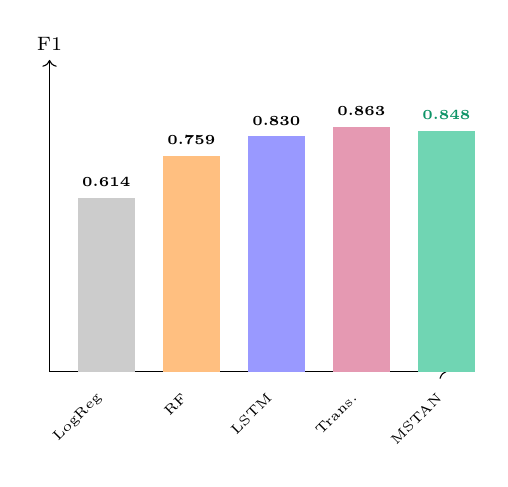
\begin{tikzpicture}[scale=0.72]
    \draw[->] (0,0) -- (0,5.5) node[above, font=\scriptsize] {F1};
    \draw[->] (0,0) -- (7,0);
    
    % Bars
    \fill[gray!40] (0.5,0) rectangle (1.5, 3.07);
    \fill[orange!50] (2,0) rectangle (3, 3.80);
    \fill[blue!40] (3.5,0) rectangle (4.5, 4.15);
    \fill[purple!40] (5,0) rectangle (6, 4.31);
    \fill[MSTANgreen!60] (6.5,0) rectangle (7.5, 4.24);
    
    % Labels
    \node[font=\tiny, rotate=45, anchor=east] at (1, -0.3) {LogReg};
    \node[font=\tiny, rotate=45, anchor=east] at (2.5, -0.3) {RF};
    \node[font=\tiny, rotate=45, anchor=east] at (4, -0.3) {LSTM};
    \node[font=\tiny, rotate=45, anchor=east] at (5.5, -0.3) {Trans.};
    \node[font=\tiny, rotate=45, anchor=east] at (7, -0.3) {MSTAN};
    
    % Values
    \node[font=\tiny\bfseries] at (1, 3.35) {0.614};
    \node[font=\tiny\bfseries] at (2.5, 4.08) {0.759};
    \node[font=\tiny\bfseries] at (4, 4.43) {0.830};
    \node[font=\tiny\bfseries] at (5.5, 4.59) {0.863};
    \node[font=\tiny\bfseries, MSTANgreen!80!black] at (7, 4.52) {0.848};
\end{tikzpicture}
\end{column}
\begin{column}{0.48\textwidth}
\textbf{Key Improvements:}
\begin{itemize}
    \item MSTAN vs LogReg: \textcolor{MSTANgreen}{\textbf{+38.1\%}} F1
    \item MSTAN vs RF: \textcolor{MSTANgreen}{\textbf{+11.7\%}} F1
    \item MSTAN vs LSTM: \textcolor{MSTANgreen}{\textbf{+2.2\%}} F1
    \item All DL models: \textbf{>0.96 ROC-AUC}
\end{itemize}
\vspace{6pt}
\begin{alertblock}{Precision--Recall Balance}
\small
\begin{tabular}{lcc}
Model & Prec & Rec \\
\midrule
LSTM & 0.781 & \textbf{0.886} \\
Transformer & \textbf{0.916} & 0.815 \\
\textbf{MSTAN} & 0.845 & 0.851 \\
\end{tabular}
\\[4pt]
MSTAN: $|P - R| = 0.006$\\
Others: $|P - R| > 0.10$
\end{alertblock}
\end{column}
\end{columns}
\end{frame}

% ──────────────────────────────────────────────────────────────────
\begin{frame}{ROC \& Precision-Recall Curves}
\begin{columns}[c]
\begin{column}{0.48\textwidth}
\centering
% Replace with your actual figure path
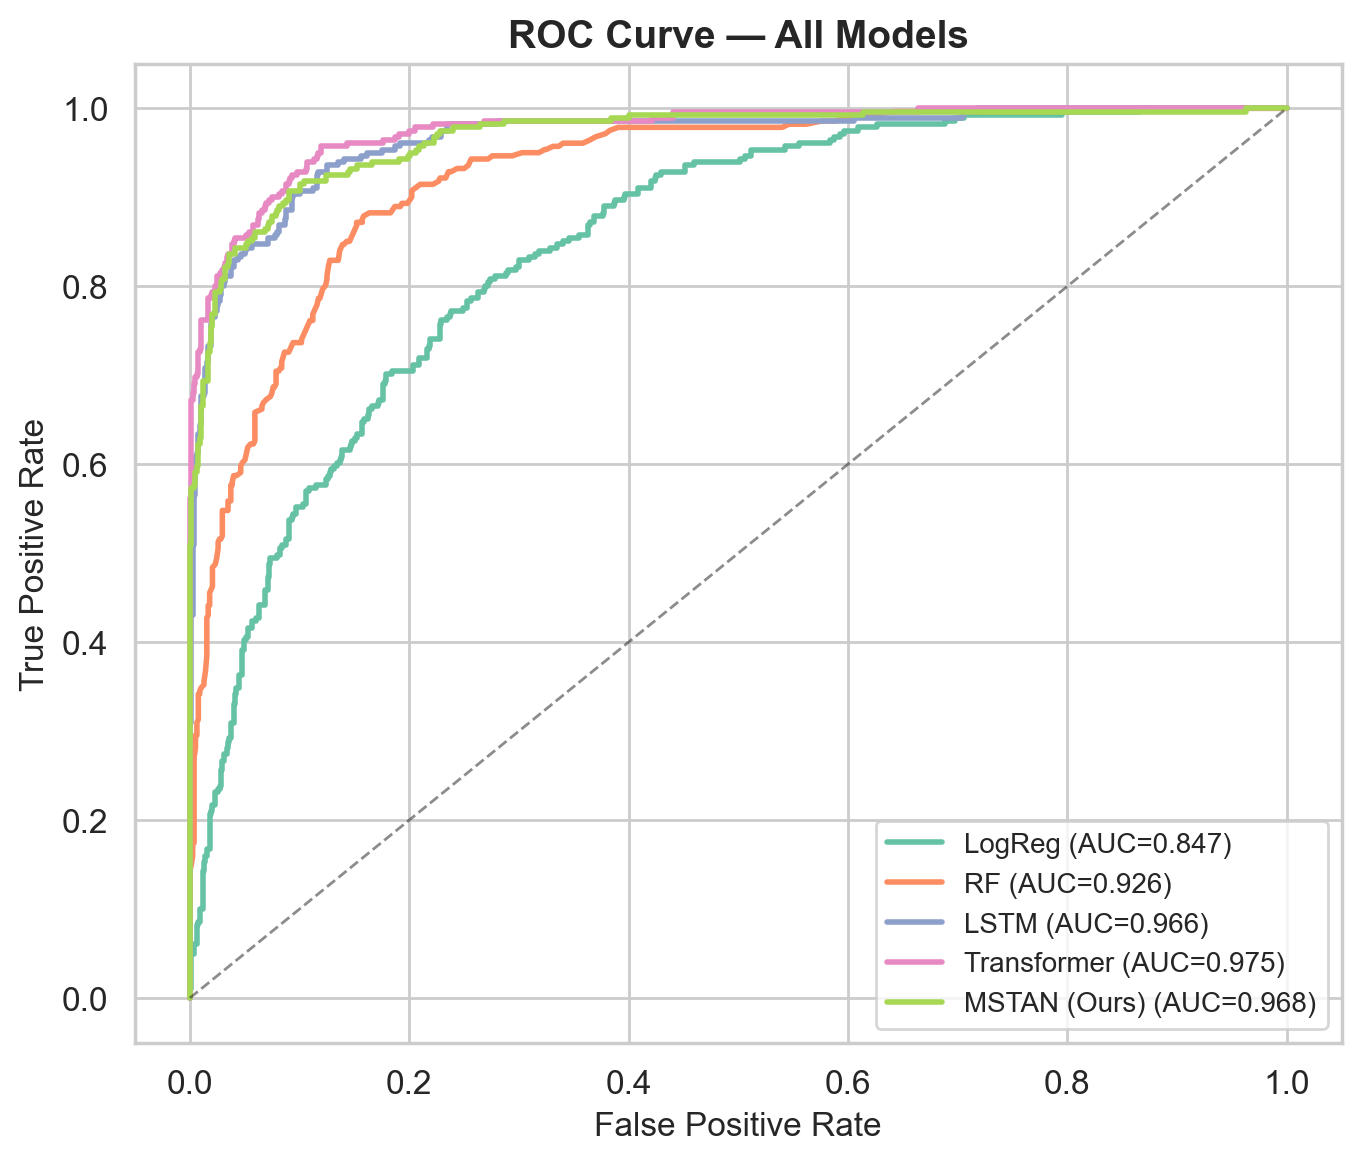
\includegraphics[width=\textwidth]{figures/multi_roc.png}
\end{column}
\begin{column}{0.48\textwidth}
\centering
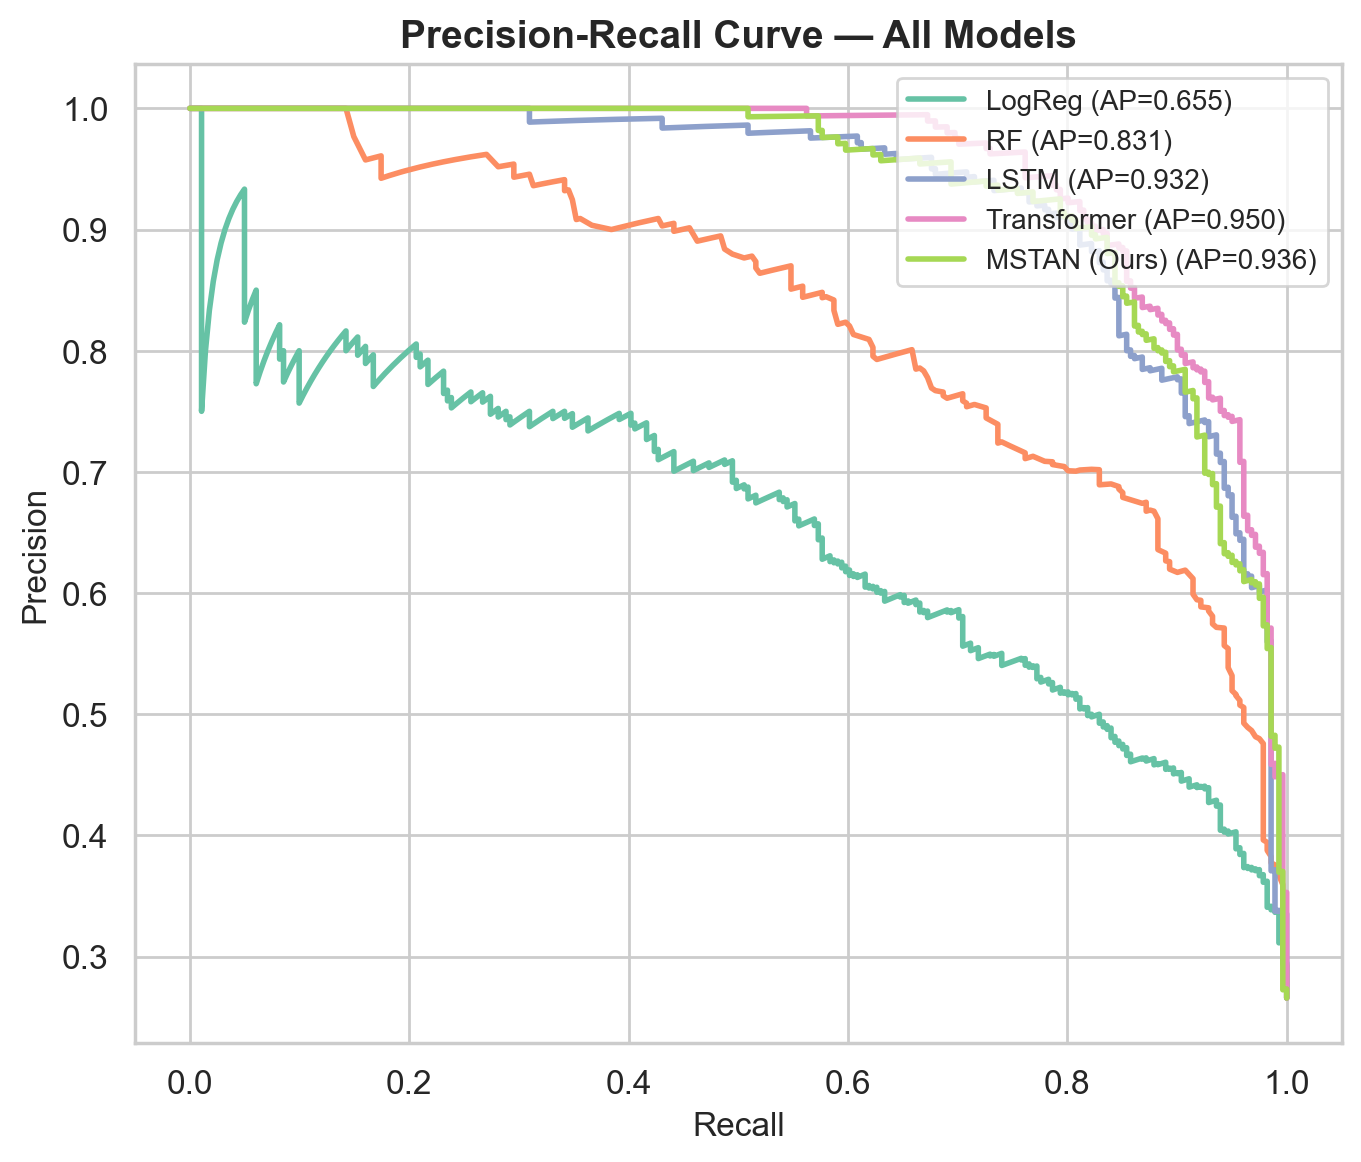
\includegraphics[width=\textwidth]{figures/multi_pr.png}
\end{column}
\end{columns}
\vspace{6pt}
\begin{itemize}
    \item All three DL models achieve \textbf{>0.96 ROC-AUC}
    \item \textbf{PR-AUC} (more informative for imbalanced data): MSTAN achieves 0.936
    \item Clear separation between DL models and traditional baselines
\end{itemize}
\end{frame}

% ──────────────────────────────────────────────────────────────────
\begin{frame}{Confusion Matrix — MSTAN}
\begin{columns}[c]
\begin{column}{0.45\textwidth}
\centering
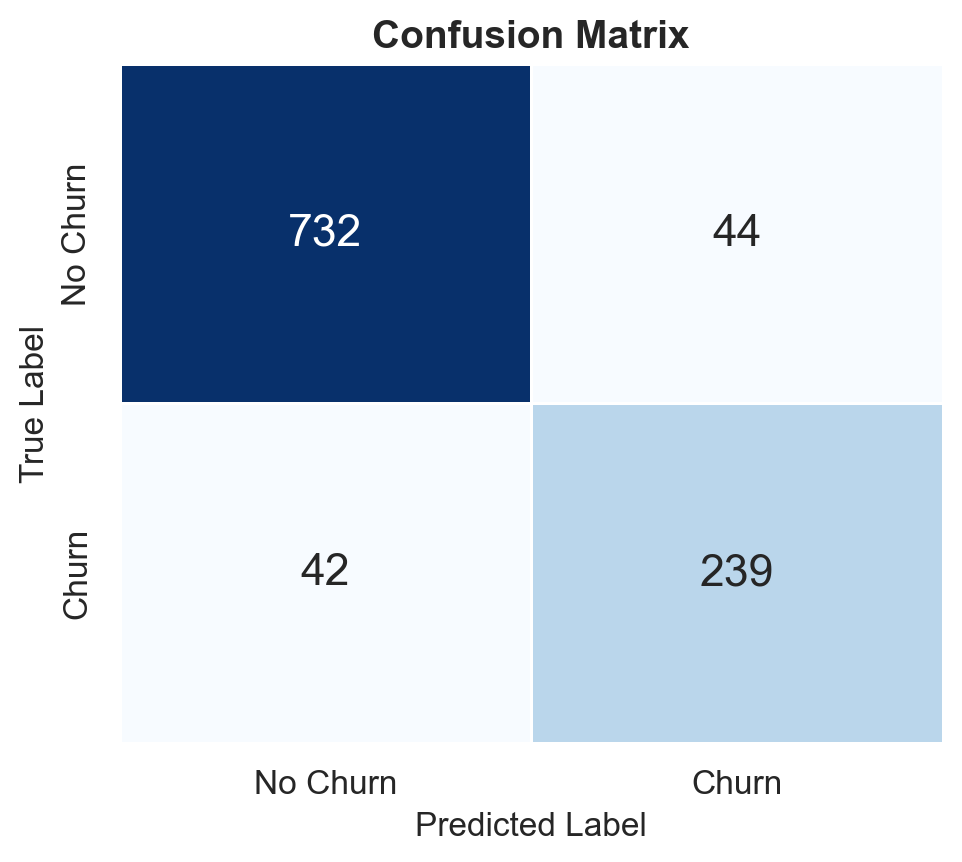
\includegraphics[width=0.95\textwidth]{figures/mstan_ours_confusion.png}
\end{column}
\begin{column}{0.52\textwidth}
\textbf{MSTAN on Test Set} (1,057 customers):
\vspace{6pt}
\begin{itemize}
    \item \textcolor{MSTANgreen}{\textbf{732}} true negatives (correctly kept)
    \item \textcolor{MSTANgreen}{\textbf{239}} true positives (correctly flagged churners)
    \item \textcolor{red}{44} false positives (unnecessary retention offers)
    \item \textcolor{red}{42} false negatives (missed churners)
\end{itemize}
\vspace{6pt}
\begin{exampleblock}{Operational Impact}
Out of 281 actual churners, MSTAN correctly identifies \textbf{239 (85.1\%)} — leaving only 42 undetected.
\end{exampleblock}
\end{column}
\end{columns}
\end{frame}

% ──────────────────────────────────────────────────────────────────
\begin{frame}{Training Dynamics}
\begin{columns}[c]
\begin{column}{0.48\textwidth}
\centering
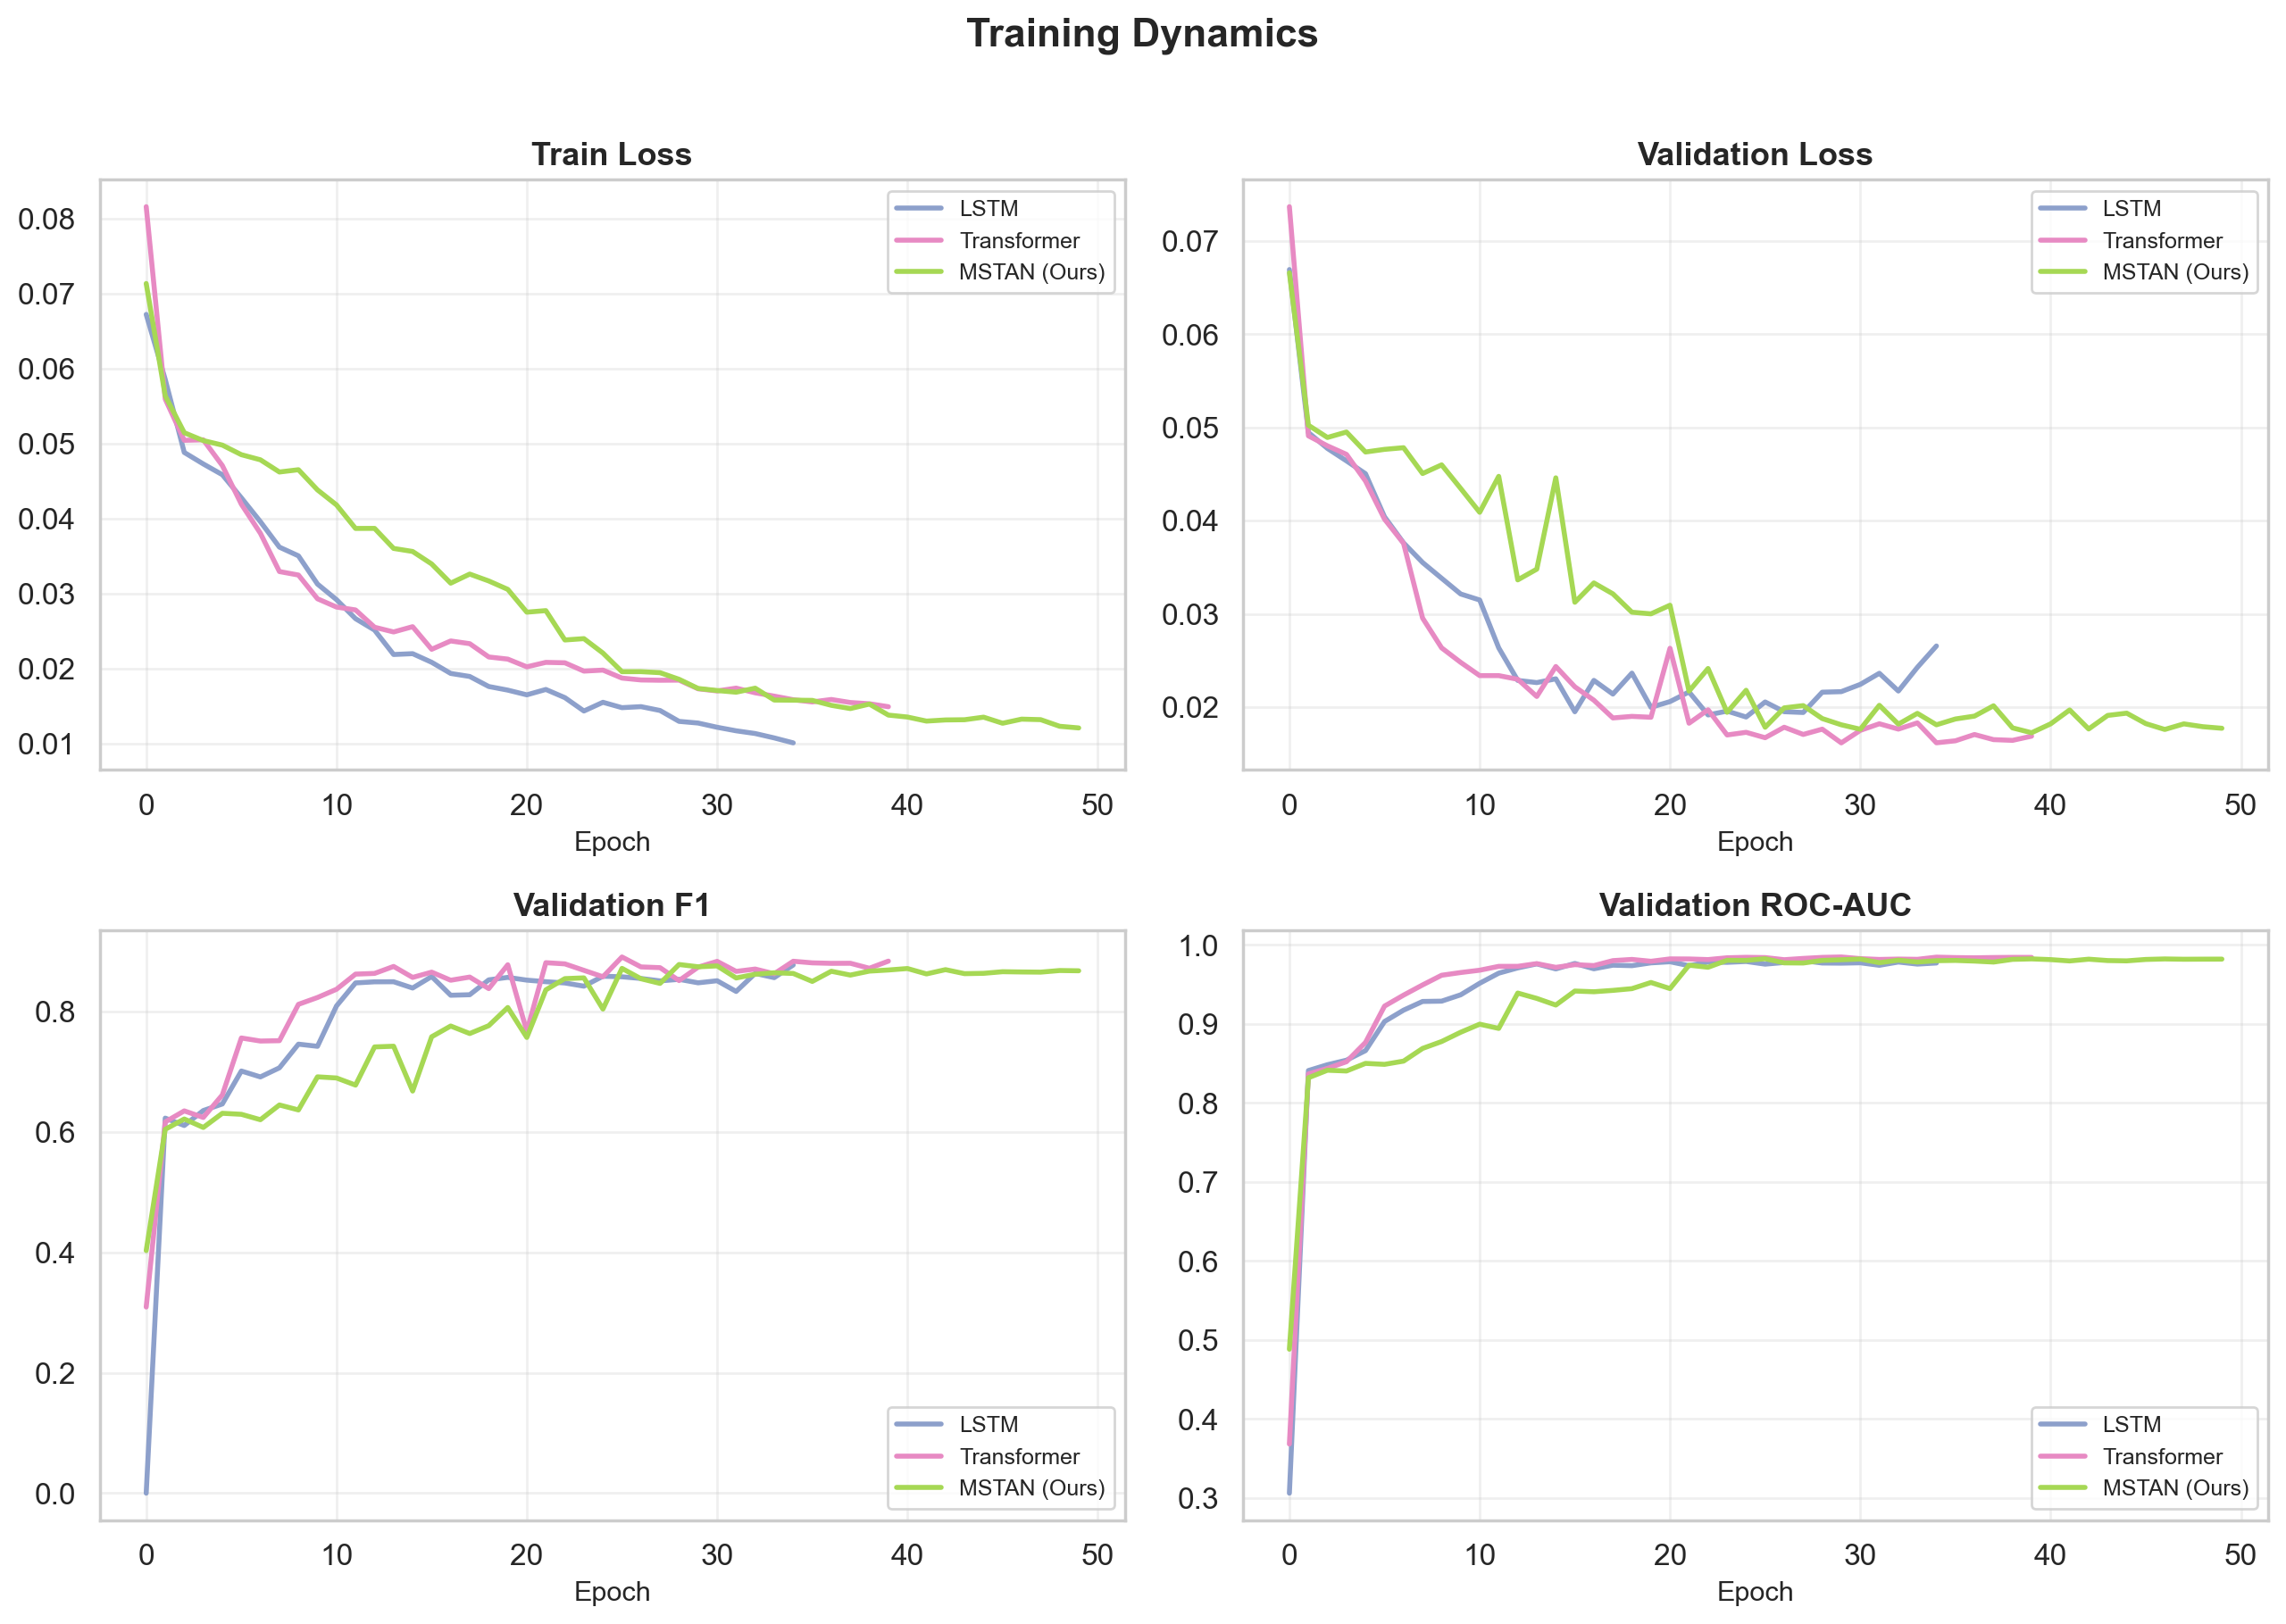
\includegraphics[width=\textwidth]{figures/training_history.png}
\end{column}
\begin{column}{0.48\textwidth}
\textbf{Observations:}
\begin{itemize}
    \item LSTM converges fastest (fewer parameters)
    \item Transformer stabilizes around epoch 25
    \item MSTAN needs \textbf{more epochs} due to multi-scale convolutions (116K params vs 70K)
    \item \textbf{Warmup scheduler} prevents early instability in MSTAN
    \item All models plateau at similar AUC ($\sim$0.98)
\end{itemize}
\vspace{4pt}
\begin{table}[h]
\centering
\scriptsize
\begin{tabular}{lc}
\toprule
\textbf{Model} & \textbf{Parameters} \\
\midrule
LSTM & 69,633 \\
Transformer & 70,081 \\
\textbf{MSTAN} & \textbf{116,556} \\
\bottomrule
\end{tabular}
\end{table}
\end{column}
\end{columns}
\end{frame}

% ══════════════════════════════════════════════════════════════════
\section{Deployment}
% ══════════════════════════════════════════════════════════════════

\begin{frame}{Interactive Dashboard}
\begin{columns}[T]
\begin{column}{0.50\textwidth}
\textbf{Technology Stack:}
\begin{itemize}
    \item \textbf{Backend:} FastAPI (Python)
    \item \textbf{Frontend:} HTML5 + Tailwind CSS + Chart.js
    \item \textbf{Model serving:} PyTorch inference
    \item \textbf{Visualizations:} Interactive charts with hover tooltips
\end{itemize}
\vspace{6pt}
\textbf{Features:}
\begin{itemize}
    \item Interactive model comparison charts
    \item Real-time churn prediction form
    \item Animated probability gauge
    \item Tabbed confusion matrix viewer
    \item Training dynamics visualization
\end{itemize}
\end{column}
\begin{column}{0.47\textwidth}
\centering
\textbf{Dashboard Preview}\\[4pt]
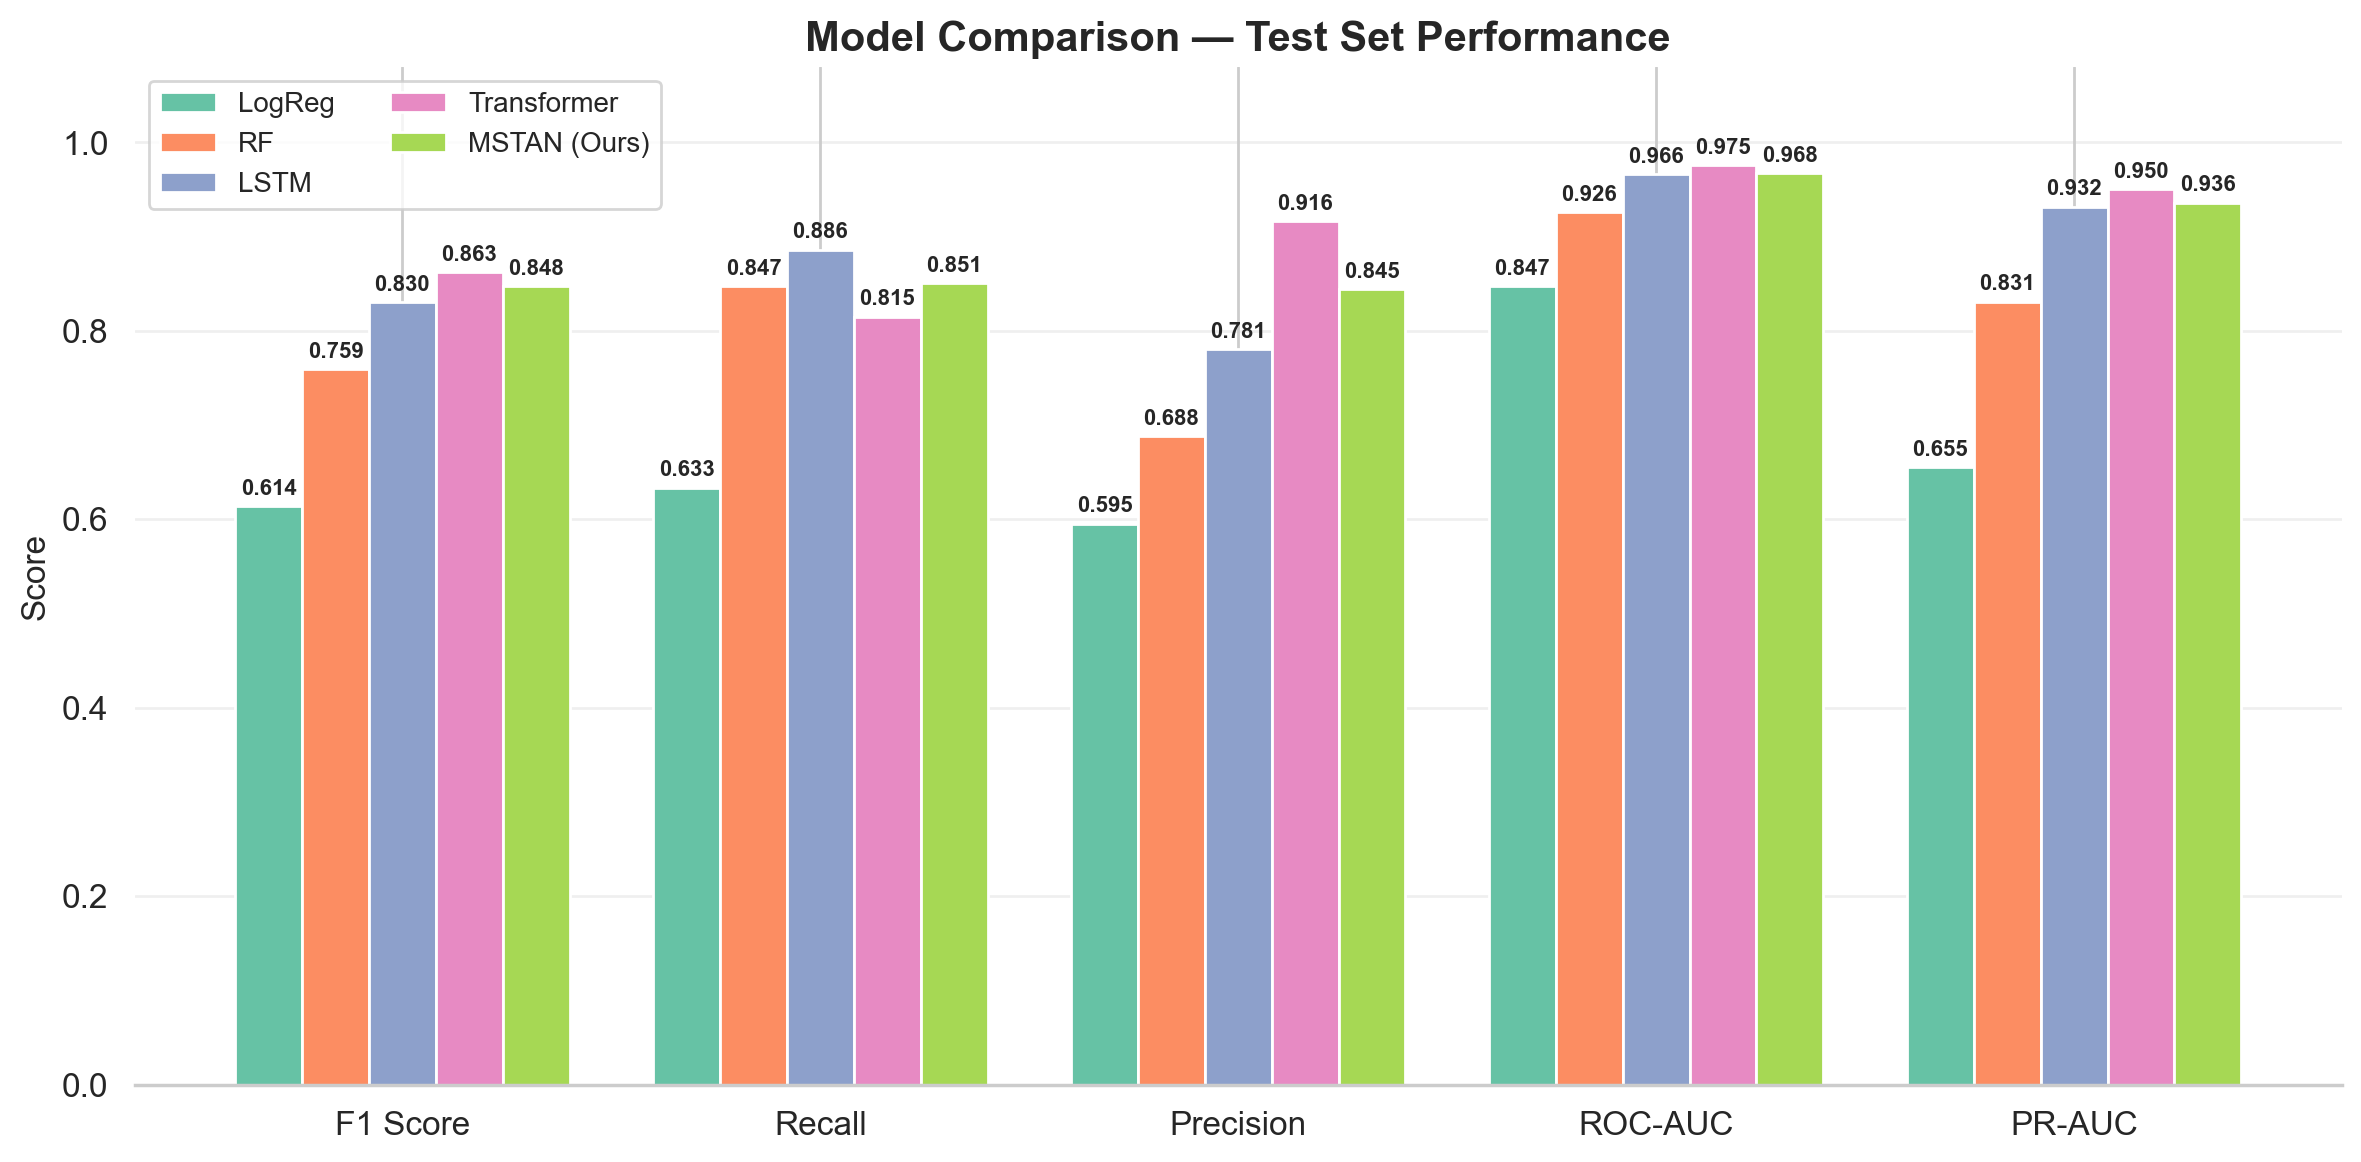
\includegraphics[width=\textwidth]{figures/comparison_bar.png}
\\[4pt]
{\scriptsize Model Comparison — Bar Chart}
\end{column}
\end{columns}
\vspace{4pt}
\centering
\texttt{uvicorn src.api.main:app -{}-port 8000} $\rightarrow$ \texttt{http://localhost:8000}
\end{frame}

% ══════════════════════════════════════════════════════════════════
\section{Conclusion \& Future Work}
% ══════════════════════════════════════════════════════════════════

\begin{frame}{Conclusion}
\begin{enumerate}
    \item We proposed \textbf{MSTAN} — a novel architecture combining multi-scale temporal convolutions with gated fusion and \emph{learnable} temporal decay attention for customer churn prediction.
    \vspace{4pt}
    \item MSTAN achieves \textbf{0.848 F1} and \textbf{0.968 ROC-AUC} with the \textbf{most balanced precision--recall trade-off} among all models tested.
    \vspace{4pt}
    \item \textbf{Focal Loss} and \textbf{F1-optimal threshold selection} significantly improve minority class detection (recall: 0.633 $\rightarrow$ 0.851).
    \vspace{4pt}
    \item The complete system includes a \textbf{one-click training pipeline} and an \textbf{interactive deployment dashboard} for real-time prediction.
\end{enumerate}
\end{frame}

% ──────────────────────────────────────────────────────────────────
\begin{frame}{Future Work}
\begin{columns}[T]
\begin{column}{0.48\textwidth}
\textbf{Technical Extensions:}
\begin{itemize}
    \item Apply MSTAN on \textbf{real longitudinal data} (e.g., CRM event logs) instead of synthesized sequences
    \item Add \textbf{SHAP-based feature importance} for local model interpretability
    \item Explore \textbf{contrastive learning} for pre-training temporal representations
\end{itemize}
\end{column}
\begin{column}{0.48\textwidth}
\textbf{Domain Extensions:}
\begin{itemize}
    \item Adapt to \textbf{other industries}: banking, SaaS, insurance
    \item Integrate with \textbf{retention cost optimization} — predict not just \emph{who} will churn but \emph{which intervention} is most cost-effective
    \item Multi-task learning: churn + \textbf{customer lifetime value} prediction
\end{itemize}
\end{column}
\end{columns}
\end{frame}

% ══════════════════════════════════════════════════════════════════
\section*{References}
% ══════════════════════════════════════════════════════════════════

\begin{frame}[allowframebreaks]{References}
\scriptsize
\begin{thebibliography}{12}
\bibitem{reichheld1996} F.\ F.\ Reichheld, \emph{The Loyalty Effect}. Harvard Business School Press, 1996.

\bibitem{vaswani2017} A.\ Vaswani et al., ``Attention Is All You Need,'' \emph{NeurIPS}, 2017.

\bibitem{bai2018} S.\ Bai, J.\ Z.\ Kolter, and V.\ Koltun, ``An Empirical Evaluation of Generic Convolutional and Recurrent Networks for Sequence Modeling,'' \emph{arXiv:1803.01271}, 2018.

\bibitem{fawaz2020} H.\ I.\ Fawaz et al., ``InceptionTime: Finding AlexNet for Time Series Classification,'' \emph{Data Mining and Knowledge Discovery}, vol.\ 34, no.\ 6, 2020.

\bibitem{press2022} O.\ Press, N.\ Smith, and M.\ Lewis, ``Train Short, Test Long: Attention with Linear Biases Enables Input Length Generalization,'' \emph{ICLR}, 2022.

\bibitem{lin2017} T.-Y.\ Lin et al., ``Focal Loss for Dense Object Detection,'' \emph{ICCV}, 2017.

\bibitem{fujo2022} S.\ Wael Fujo, S.\ Subramanian, and A.\ H.\ Khader, ``Customer Churn Prediction in Telecommunication Industry Using Deep Learning,'' \emph{Information Sciences}, vol.\ 597, 2022.

\bibitem{amin2019} A.\ Amin et al., ``Customer Churn Prediction in Telecommunication Industry Using Data Certainty,'' \emph{Journal of Business Research}, vol.\ 94, 2019.

\bibitem{decaigny2018} A.\ De Caigny, K.\ Coussement, and K.\ W.\ De Bock, ``A New Hybrid Classification Algorithm for Customer Churn Prediction,'' \emph{European J. of Operational Research}, vol.\ 269, no.\ 2, 2018.

\bibitem{lalwani2022} P.\ Lalwani et al., ``Customer Churn Prediction System: A Machine Learning Approach,'' \emph{Computing}, vol.\ 104, no.\ 2, 2022.

\bibitem{wen2023} Q.\ Wen et al., ``Transformers in Time Series: A Survey,'' \emph{IJCAI}, 2023.

\bibitem{lim2021} B.\ Lim et al., ``Temporal Fusion Transformers for Interpretable Multi-horizon Time Series Forecasting,'' \emph{Int.\ J.\ of Forecasting}, vol.\ 37, no.\ 4, 2021.
\end{thebibliography}
\end{frame}

% ══════════════════════════════════════════════════════════════════

\begin{frame}[plain]
\begin{center}
\vspace{2cm}
{\Huge\bfseries Thank You}\\[12pt]
{\large Questions?}\\[20pt]
{\small\color{gray} Source Code: \texttt{github.com/51riu5/churn\_ai}}\\[4pt]
{\small\color{gray} Dashboard: \texttt{http://localhost:8000}}
\end{center}
\end{frame}

\end{document}
